\documentclass[10pt, a4paper, landscape, xcolor=dvipsnames]{extarticle}
\pagestyle{empty} % Keine Seitennummern

% Verwendete Pakete

	\usepackage[utf8]{inputenc}
	\usepackage[top=0.7cm, bottom=0.9cm, left=0.65 cm, right=0.65 cm, ]{geometry}
	\usepackage{amsmath}
	\usepackage{amsfonts}
	\usepackage{lmodern}
	\usepackage{graphicx}
	\setlength{\parindent}{0pt}
	\usepackage[normalem]{ulem}
	\usepackage[dvipsnames]{xcolor}
	\usepackage{enumitem}
	\usepackage{mathabx}
	\usepackage{enumitem}
	\usepackage{colortbl}
	\usepackage[ngerman]{babel}
	\usepackage{mathtools}
	\usepackage{wallpaper}
	\usepackage{changepage}
	\usepackage{tikz}
	\usepackage{tabularx}
	\usepackage{tcolorbox}
	\usepackage{lipsum}
	\usepackage{multicol}
	\usepackage{letltxmacro}
	\usepackage{tabularx}
	\usepackage{multicol}
	\usepackage{multicol}
	\usepackage{calc}
	\usepackage{ifthen}
	\usepackage{hyperref}
	\usepackage{graphicx}
	\graphicspath{ {./img/} }
	\usepackage{wrapfig}


% Spalteneinstellungen

	\setlength\columnsep{3mm}
	\setlength{\columnseprule}{0pt}
	
% Neue Befehle

	% Bullet-Symbol für Aufzählungen
	\renewcommand\textbullet{\ensuremath{\bullet}}
	
	% Eingekreiste Nummern für Aufzählungen
	\newcommand*\circled[1]{\tikz[baseline=(char.base)]{
            \node[shape=circle,draw,inner sep=1.2pt] (char) {#1};}}
            
    % Horizontale Punkte
    \LetLtxMacro\orgddots\ddots
    \makeatletter
	\DeclareRobustCommand\vdots{%
	  \mathpalette\@vdots{}%
	}
	\newcommand*{\@vdots}[2]{%
	  % #1: math style
	  % #2: unused
	  \sbox0{$#1\cdotp\cdotp\cdotp\m@th$}%
	  \sbox2{$#1.\m@th$}%
	  \vbox{%
	    \dimen@=\wd0 %
	    \advance\dimen@ -3\ht2 %
	    \kern.5\dimen@
	    % remove side bearings
	    \dimen@=\wd2 %
	    \advance\dimen@ -\ht2 %
	    \dimen2=\wd0 %
	    \advance\dimen2 -\dimen@
	    \vbox to \dimen2{%
	      \offinterlineskip
	      \copy2 \vfill\copy2 \vfill\copy2 %
	    }%
	   }%
	}
	\DeclareRobustCommand\ddots{%
		\mathinner{%
		   \mathpalette\@ddots{}%
		   \mkern\thinmuskip
		}%
	}
	
	% Vertikale Punkte
	\DeclareRobustCommand\ddots{%
		  \mathinner{%
		    \mathpalette\@ddots{}%
		    \mkern\thinmuskip
		  }%
		}
		\newcommand*{\@ddots}[2]{%
		  % #1: math style
		  % #2: unused
		  \sbox0{$#1\cdotp\cdotp\cdotp\m@th$}%
		  \sbox2{$#1.\m@th$}%
		  \vbox{%
		    \dimen@=\wd0 %
		    \advance\dimen@ -3\ht2 %
		    \kern.5\dimen@
		    % remove side bearings
		    \dimen@=\wd2 %
		    \advance\dimen@ -\ht2 %
		    \dimen2=\wd0 %
		    \advance\dimen2 -\dimen@
		    \vbox to \dimen2{%
		      \offinterlineskip
		      \hbox{$#1\mathpunct{.}\m@th$}%
		      \vfill
		      \hbox{$#1\mathpunct{\kern\wd2}\mathpunct{.}\m@th$}%
		      \vfill
		      \hbox{$#1\mathpunct{\kern\wd2}\mathpunct{\kern\wd2}\mathpunct{.}\m@th$}%
		    }%
		  }%
		}
	\makeatother
	
	% Schriftart
	\renewcommand{\familydefault}{\sfdefault}
	
	% Dokument-Info Block	
	\newcommand{\DocumentInfo}[3]{
	\begin{tcolorbox}[
			arc=0mm, 
			colback = white!38!black,
			boxrule=0pt,
			toptitle=1mm,
			bottomtitle=1mm,
			right=2mm,
			left=2mm,
			leftright skip = -0.5mm,
			title= \huge \center \textbf{#1} \par \large \vskip1mm #2 \par \vskip1mm \small 	Version: \today,
			fontupper=\color{white},
			after skip = 0 mm,
			top=0.1mm,
			bottom=1mm]
		
		\small #3
	\vskip1mm	
	\end{tcolorbox}
	}
	
	% Überschrift
	\renewcommand{\section}[1]{
	\begin{tcolorbox}[
			arc=0mm,
			colback=white!38!black,
			colframe=white,
			bottomrule = 0 mm,
			toprule = 0 mm,
			leftrule = 0 mm,
			rightrule = 0 mm,
			valign=center,
			left=0.5mm,
			top= 0.7 mm,
			bottom= 0.7 mm,
			fontupper=\color{white},
			before skip = 0mm,
			leftright skip = -0.5mm,
			after skip = 0 mm]

		\textbf{#1}
	\end{tcolorbox}
	}
	
	% Abschnitt	
	\renewcommand{\subsection}[2]{
	\begin{tcolorbox}[
			arc=0mm,
			colback=white!75!black,
			colframe=white,
			bottomrule = 0 mm,
			toprule = 0 mm,
			leftrule = 0 mm,
			rightrule = 0 mm,
			valign=center,
			left=0.5mm,
			top=0.2mm,
			bottom=0.2mm,
			before skip = 0mm,
			leftright skip = -0.5mm,
			after skip = 1.4 mm]
			
		\small \textbf{#1}
	\end{tcolorbox}
	
	\begin{adjustwidth}{0.5mm}{1mm}
		\small
		#2
		\vspace{0.5mm}
	\end{adjustwidth}
	}
	
	% Weisser Balken zwischen Abschnitten
	\newcommand{\WhiteSpace}[0]{
	\begin{tcolorbox}[
			arc=0mm,
			colback=white,
			colframe=white,
			bottomrule = 0 mm,
			toprule = 0 mm,
			leftrule = 0 mm,
			rightrule = 0 mm,
			valign=center,
			left=0.5mm,
			top= -0.2 mm,
			bottom= -0.2 mm,
			fontupper=\color{white},
			before skip = 0mm,
			leftright skip = -0.5mm,
			after skip = 0 mm]
	
	\end{tcolorbox}
	}
	
% Hintergrundbild (graue Spalten)

%	\CenterWallPaper{1}{0_Setup/background.pdf}

% TabularX Zeug (Paket für Tabellen)

	\newcolumntype{C}[1]{>{\centering\arraybackslash}p{#1}}

% TikZ Zeug (Paket für Vektorgraphiken)

	\usetikzlibrary{decorations.pathreplacing,calc}

	\newcommand{\tikzmark}[2][-3pt]{\tikz[remember picture, overlay, baseline=-0.5ex]\node[#1](#2){};}
	
	\tikzset{brace/.style={decorate, decoration={brace}},
	 brace mirrored/.style={decorate, decoration={brace,mirror}},
	}
	
	\newcounter{brace}
	\setcounter{brace}{0}
	\newcommand{\drawbrace}[3][brace]{%
	 \refstepcounter{brace}
	 \tikz[remember picture, overlay]\draw[#1] (#2.center)--(#3.center)node[pos=0.5, name=brace-\thebrace]{};
	}
	
	\newcommand{\annote}[3][]{%
	 \tikz[remember picture, overlay]\node[#1] at (#2) {#3};
	}

\begin{document}

% Vier Spalten
\begin{multicols*}{3}

    % Info über das Dokument
    \DocumentInfo
    {Lineare Algebra S2} %Titel
    {Raphael Nambiar} %Untertitel

    \WhiteSpace

    % Dokumentinhalt
    \section{Vektorgeometrie}
    \subsection{Begriffe}
    {\textbf{Kollinear:} Es existiert eine Gerade $g$, zu der beide Vektoren parallel sind.}
    {\textbf{Komplanar:} Existiert eine Ebene $e$, zu der alle drei Vektoren parallel.}

    {\textbf{Ortsvektor:} Beginnt vim Ursprung. Schreibweise: $\vec{r}(P) $}

    {\textbf{Nullvektor:} Vektor mit Betrag 0,keine Richtung.:  $\vec{0} $}
    \WhiteSpace
    \subsection{Betrag}
    {
        $\mid \vec{a} \mid  $ =
        $\begin{pmatrix}
                x \\
                y \\
                z
            \end{pmatrix}$ = $ \sqrt[]{x^2+y^2+z^2}$
        \WhiteSpace
        \subsection{Skalarprodukt}

        $\vec{a} \cdot \vec{b} =  \begin{pmatrix}
                a_x \\
                a_y \\
                a_z
            \end{pmatrix} \cdot \begin{pmatrix}
                b_x \\
                b_y \\
                b_z
            \end{pmatrix} = a_xb_x+a_yb_y+a_zb_z$

        $ \vec{a} \cdot \vec{b} $ = $ \mid \vec{a} \mid \cdot \mid \vec{b} \mid \cdot \cos(\varphi)$

        $\cos(\varphi) $ = $\frac{\vec{a} \cdot \vec{b}}{\mid \vec{a} \mid \cdot \mid \vec{b} \mid} \rightarrow \arccos(\frac{\vec{a} \cdot \vec{b}}{\mid \vec{a} \mid \cdot \mid \vec{b} \mid}) $
    }
    \WhiteSpace
    \subsection{Orthogonal}
    {Wenn zwei Vektoren senkrecht zueinander sind.}
    $ \vec{a} \cdot \vec{b} $ = 0
    \WhiteSpace
    \subsection{Orthogonale Projektion}
    {Projektion des Vektores $\vec{b} $ auf den Vektor $\vec{a} $.}
    \begin{multicols*}{2}
        {   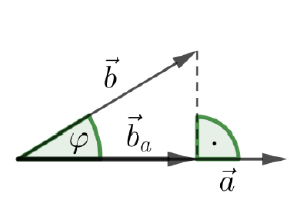
\includegraphics[scale=0.35]{ortho.png}}

        \columnbreak

        $\vec{b}_a = \frac{\vec{a} \cdot  \vec{b}}{\mid \vec{a} \mid ^2} \cdot \vec{a} $

        $\mid \vec{b}_a  \mid  = \frac{\mid \vec{a} \mid \cdot \mid \vec{b} \mid}{\mid \vec{a} \mid }$

        $ \mid \vec{b}_a \mid $ = $\mid \vec{a} \mid \cdot \cos(\varphi)$

    \end{multicols*}

    \subsection{Zwischenwinkel}
    {$\varphi = cos^{-1}(\frac{\vec{a}\cdot\vec{b}}{\mid \vec{a} \mid \cdot \mid \vec{b} \mid}) $}
    \WhiteSpace
    \subsection{Einheitsvektor}
    {$\vec{e}_a $ = $\frac{1}{\mid \vec{a} \mid} \cdot \vec{a}$ ;$\mid \vec{e}_a \mid$ = 1}
    \subsection{Vektorprodukt / Kreuzprodukt}

    \begin{multicols}{2}
        \noindent
        {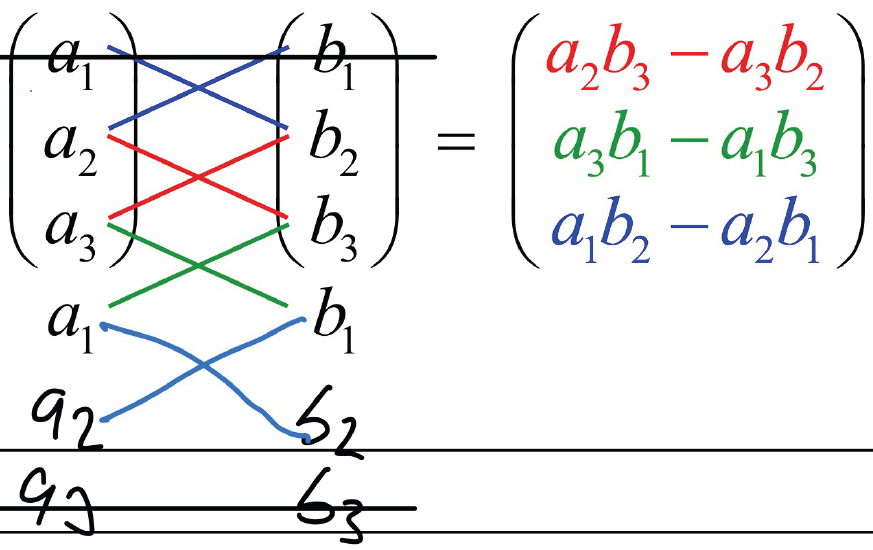
\includegraphics[scale=0.15]{vekProd.png}}
        \columnbreak

        { $ \mid \vec{a} \times \vec{b} \mid = \mid\vec{a}\mid \cdot \mid\vec{b}\mid \cdot \cos(\alpha) $}

        {$\vec{a} \times \vec{b}$ ist orthogonal zu $\vec{a}$ und zu $\vec{b}$}

    \end{multicols}
    \textbf{Kreuzprodukt in R²}

    { 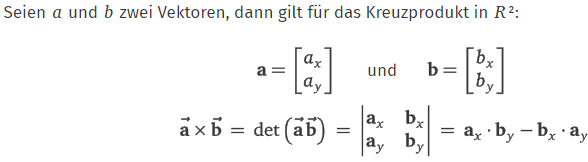
\includegraphics[scale=0.4]{vekProd_r2.png}}

    \subsection{Fläche / Parallelogramm }



    \begin{multicols}{2}

        {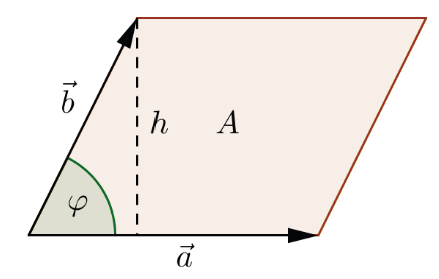
\includegraphics[scale=0.2]{vekProdParallelo.png}}

        \columnbreak

        { $\mid \vec{a} \times \vec{b} \mid $ = A }

        {Dreieck = $\frac{1}{2}$ A}

    \end{multicols}

    \subsection{Volumen / Spatprodukt }

    {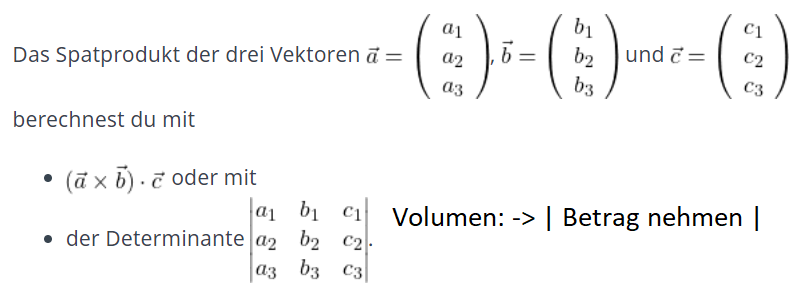
\includegraphics[scale=0.4]{spatprod.png}}
    \vfill\null
    \columnbreak
    \section{Geraden}

    \subsection{Parameterdarstellung}
    {\large $ g: \vec{r}(P) + \lambda \cdot \vec{a}  $}

    {P: Aufpunkt}

    {$ \vec{a}$ = $\overrightarrow{PQ} $;  = Richtungsvektor}


    \subsection{Koordinatendarstellung}
    {$g: ax + by + c= 0 $}
    \subsection{Koordinatendarstellung zu Parameterdarstellung }
    {Zwei Punkte auf $ g $  bestimmen: 2 beliebige x Koordinaten wählen und in $ g $ einsetzen. Danach jeweils $ y $ auslesen. Dies ergibt zwei Punkte $P,Q$. In Parameterdarstellung bringen.}

    \subsection{Parameterdarstellung zu Koordinatendarstellung}
    {Gerade $ g:  \begin{pmatrix}
                7 \\
                1
            \end{pmatrix} + \lambda \cdot \begin{pmatrix}
                -2 \\
                -4
            \end{pmatrix} $ }
    {Gleichungssystem aufstellen und Lösen:}
    \begin{gather*}
        x = 7 - 2 \lambda \\
        y = 1 - 4 \lambda
    \end{gather*}
    {In Koordinatendarstellung bringen:}
    $ -2x + y + 13 = 0$

    \subsection{Abstand Punkt zu Geraden}
    { Gerade g: $ \begin{pmatrix}
                1  \\
                13 \\
                -5
            \end{pmatrix} + \lambda \cdot
            \begin{pmatrix}
                3 \\
                5 \\
                -4
            \end{pmatrix} $}

    {Punkt A: $(3,-1,4)$}

    {$\overrightarrow{PA}$ = $\begin{pmatrix}
                3  \\
                -1 \\
                4
            \end{pmatrix} -  \begin{pmatrix}
                1  \\
                13 \\
                -5
            \end{pmatrix} =
            \begin{pmatrix}
                2   \\
                -14 \\
                9
            \end{pmatrix} $}

    {$l = \frac {\mid \overrightarrow{PA} \times\vec{a}\mid}{\mid\vec{a}\mid} $}

    {\small $\vec{a} \Rightarrow $  aus der Parameterdarstellung}
    \vfill\null
    \columnbreak
    \section{Ebene}

    \subsection{Normalenvektor der Ebene (orthogonal zur Ebene)}
    {Auf der Ebene $ E $ senkrecht stehnder Vektor $\vec{n}$.}
    $\vec{n} = \vec{a} \times \vec{b}$
    \WhiteSpace
    \subsection{Parameterdarstellung}
    {\large $ E: \vec{r}(P) + \lambda \cdot \vec{a} + \mu \cdot \vec{b} $}
    {P: Aufpunkt}

    {$ \vec{a}$ = $\overrightarrow{PQ} $; $ \vec{b}$ = $\overrightarrow{PR} $ = Richtungsvektoren}
    \WhiteSpace
    \subsection{Koordinatendarstellung}
    {$E: ax + by + cz + d = 0 $}

    \subsection{Parameterdarstellung zu Koordinatendarstellung}
    { $ E: \begin{pmatrix}
                2 \\
                4 \\
                1
            \end{pmatrix} + \lambda \cdot
            \begin{pmatrix}
                1 \\
                3 \\
                1
            \end{pmatrix} + \mu \cdot
            \begin{pmatrix}
                2 \\
                4 \\
                -4
            \end{pmatrix}$

        $\vec{n}=
            \begin{pmatrix}
                1 \\
                3 \\
                1
            \end{pmatrix} \times \begin{pmatrix}
                2 \\
                4 \\
                -4
            \end{pmatrix} = \begin{pmatrix}
                -14 \\
                6   \\
                -4
            \end{pmatrix} $}

    \circled{2} Koordinatendarstellung $ E: -14x + 6y - 4z + d = 0$

    \circled{3} Aufpunkt einsetzen: $\begin{pmatrix}
            2 \\
            4 \\
            1
        \end{pmatrix} 	\Rightarrow  E: -14 \cdot 2  + 6 \cdot 4 - 4\cdot 1 + d = 0 $

    \circled{4} $d$ ausrechnen: $ E: -14 \cdot 2  + 6 \cdot 4 - 4\cdot 1 + d = 0 \Rightarrow d = 8$

    \circled{5} $E: -14x + 6y - 4z + 8 = 0$

    $\Rightarrow \frac{-14x + 6y - 4z + 8 = 0}{2} \Rightarrow E: -7x + 3y - 2z + 4 = 0$

    \subsection{Koordinatendarstellung zu Parameterdarstellung }
    {Wir bestimmen drei beliebige Punkte auf $ E$, indem wir die $x$- und $y$-Koordinaten frei wählen
        und die zugehörigen $z$-Koordinaten aus der Koordinatendarstellung von $E$ berechnen. Aus
        diesen drei Punkten können wir dann eine Parameterdarstellung von $E$ gewinnen.}
    {$E: 2x + 7y -4z + 1 = 0$}

    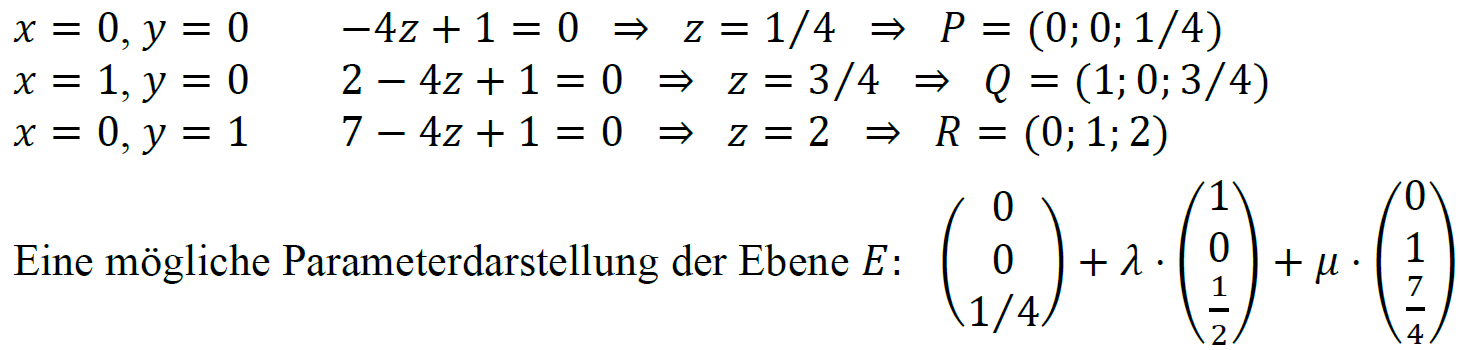
\includegraphics[scale=0.2]{koord_to_param.png}

    \subsection{Abstand Punkt zu Ebene}
    {Abstand \Large $  l = \frac{\mid ax_A + bx_A + cz_A + d  \mid}{\mid \vec{n} \mid}$ }
    {Ebene $E:  3x-6y-2z+67=0 $}

    {Punkt $A = (3,-4,1)$}


    {\circled{1} $\vec{n}$ bestimmen: $\begin{pmatrix}
                3  \\
                -6 \\
                -2
            \end{pmatrix}$ $\sqrt{3^2+-6^2+-2^2} = 7$}

    {\circled{2} $l = \frac{(3 \cdot 3) -(6 \cdot (-4)) - (2 \cdot 1)}{7} = 14$}
    \WhiteSpace


    \subsection{  normierte Koordinatendarstellung der Ebene}
    {$E: 2x + 7y - 4z + 1 = 0$}
    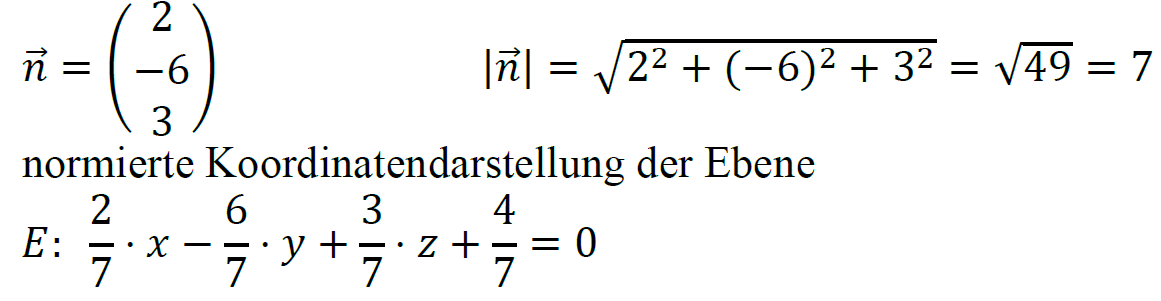
\includegraphics[scale=0.2]{normiert.png}

    \vfill\null
    \columnbreak
    \section{Linearen Gleichungssysteme}
    \WhiteSpace
    \subsection{Rang}
    {Matrix muss in Zeilenstufenform sein.}

    {$rg(A) = $ Gesamtanzahl Zeilen - Anzahl Nullzeilen .}

    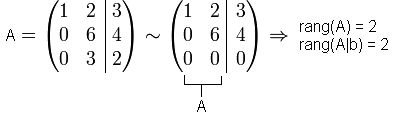
\includegraphics[scale=0.75]{rang.png}

    \subsection{Lösbarkeit von LGS}
    {$ n $ = Anzahl Spalten(Variablen)}
    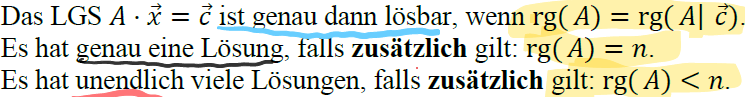
\includegraphics[scale=0.45]{loesbarkeit.png}
    \subsection{Freie Variable}

    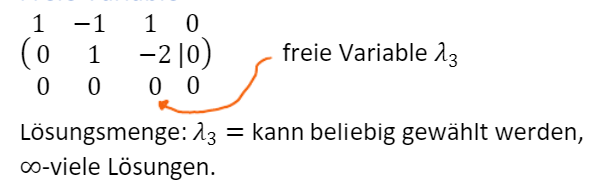
\includegraphics[scale=0.75]{free_vars.png}

    \vfill\null
    \columnbreak
    \section{Matrizen}
    \subsection{Begriffe}
    {\textbf{Quadratische Matrix:} gleich viele Zeilen und Spalten}

    \textbf{Hauptdiagonale:} Die Diagonale von links oben nach rechts unten

    \textbf{Untere- und obere Dreiecksmatrix}

    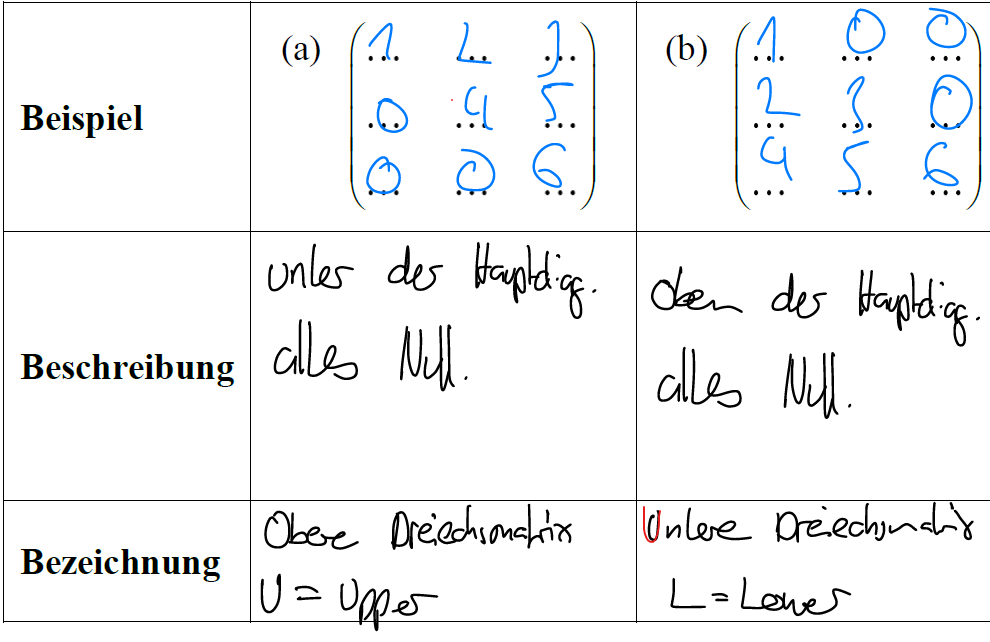
\includegraphics[scale=0.25]{untere_obere.png}

    \textbf{Symmetrische Matrix :} symmetrisch bzgl. Hauptdiagonale

    $ \begin{pmatrix}
            1 & 5 & 6 \\
            5 & 2 & 3 \\
            6 & 3 & 1
        \end{pmatrix} $

    \WhiteSpace
    \subsection{Multiplikation / Rechenregeln}
    {\begin{multicols}{2}
            { 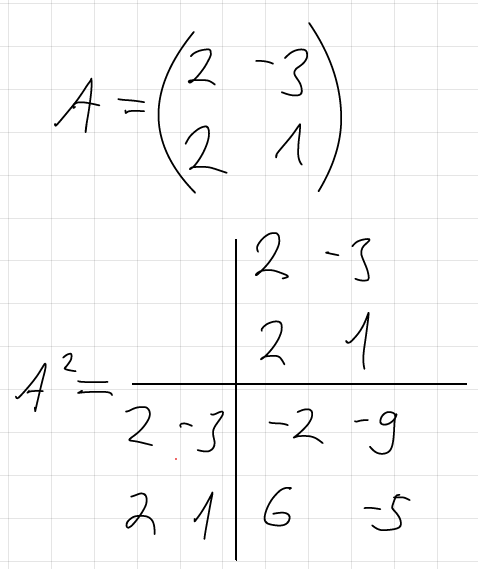
\includegraphics[scale=0.25]{matrix_multi.png} }
            \columnbreak
            { 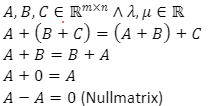
\includegraphics[scale=0.8]{rechenregeln.png} }
        \end{multicols}}

    \subsection{Transponieren}

    A = $\begin{pmatrix} {\color{red}2} & {\color{red}3} & {\color{red}0} \\ 1 & 4 & 5 \end{pmatrix} \quad
        \rightarrow
        \quad A^{T} = \begin{pmatrix} {\color{red}2} & 1 \\ {\color{red}3} & 4 \\ {\color{red}0} & 5 \end{pmatrix}
    $

    {Rechenregeln:}

    $ \left(A^{T}\right)^{T} = A $

    $ \left(A + B\right)^{T} = A^{T} + B^{T} $

    $ \left(A \cdot B\right)^{T} = B^{T} \cdot A^{T} $

    {Gilt $ A = A^{T} $, so heißt die Matrix A symmetrisch.}


    {Gilt $ A = -A^{T} $, so heißt die Matrix A antisymmetrisch.}
    \vfill\null
    \columnbreak
    \subsection{Inverse}
    {Matrix muss quadratisch sein$: n \times n \rightarrow 2\times2, 3\times3$}

    \textbf{2x2}

    {\large$\begin{pmatrix}
            a & b \\
            c & d
        \end{pmatrix}^{-1} = \frac{1}{ad-bc}\cdot\begin{pmatrix}
            d  & -b \\
            -c & a
        \end{pmatrix}$}

    {Die $2\times2$-Matrix hat genau dann ein Invese wenn $ad-bc \neq 0$}

    \textbf{3x3 und grösser}

    {$\rightarrow$ Gauss - Jordan}

    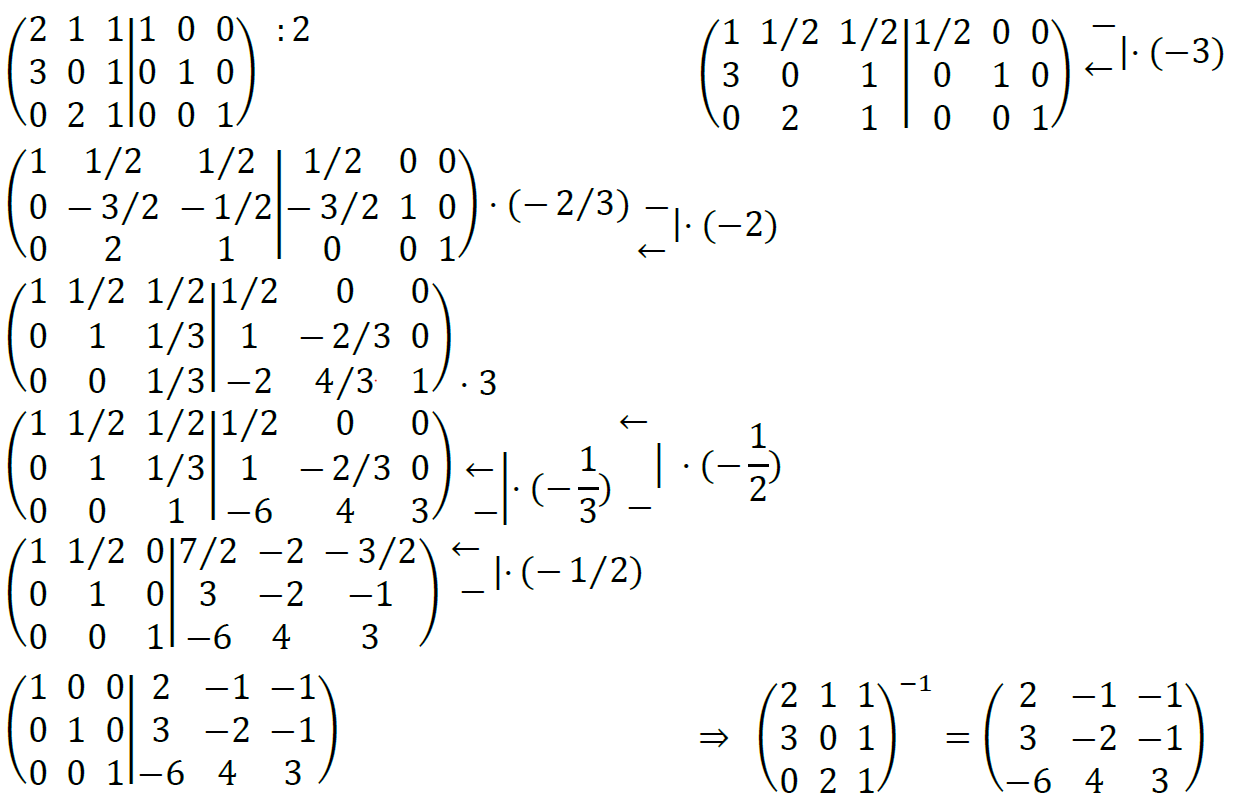
\includegraphics[scale=0.25]{3x3_inverse.png}
    \WhiteSpace

    \subsection{Determinante}
    {\textbf{2x2}}

    $\begin{vmatrix}
            a & b \\
            c & d
        \end{vmatrix} = a\cdot d - b\cdot c $
    \WhiteSpace
    \textbf{3x3 Regel von Sarrus}

    $\begin{vmatrix} a & b & c \\ d & e & f \\ g & h &i \end{vmatrix} = a \cdot e \cdot i + b \cdot f \cdot g + c \cdot d \cdot h - g \cdot e \cdot c - h \cdot f \cdot a - i \cdot d \cdot b.$
    \WhiteSpace
    \textbf{Laplacescher Entwicklungssatz ($ >$3x3)}

    {\begin{multicols}{2}
            Vorzeichen:

            \columnbreak
            { 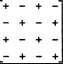
\includegraphics[scale=0.75]{checkerboard.png} }

        \end{multicols}}

    {\small{Entwickeln nach derjenigen Zeile oder Spalte, in
            der die meisten Nullen stehen (hier gelb)}}
    {\begin{multicols}{2}
            {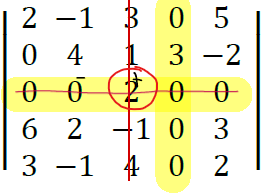
\includegraphics[scale=0.40]{laplace.png}}
            \columnbreak

            {  $ \rightarrow  2 \cdot det \begin{vmatrix} 2 & 1 & 0 & 5 \\ 0 & 4 & 3 & -2 \\ 6 & 2 &0 & 3 \\ 3 & -1 &0 & 2 \end{vmatrix} $}
        \end{multicols}}
    {\small{Wichtig: häufig sind die entwickelten identisch! $\rightarrow$ Aufwand sparen!}}
    {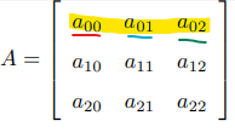
\includegraphics[scale=0.6]{laplace_full_1.png}Entwicklen nach 1er}

    {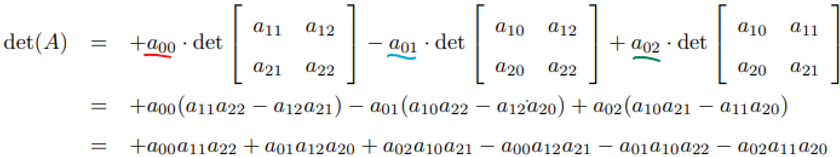
\includegraphics[scale=0.4]{laplace_full_2.png}}


    \textbf{$det$ Dreiecksmatrix}
    $ = $ Produkt der Hauptdiagonale
    \WhiteSpace

    \textbf{Rechenregeln}

    {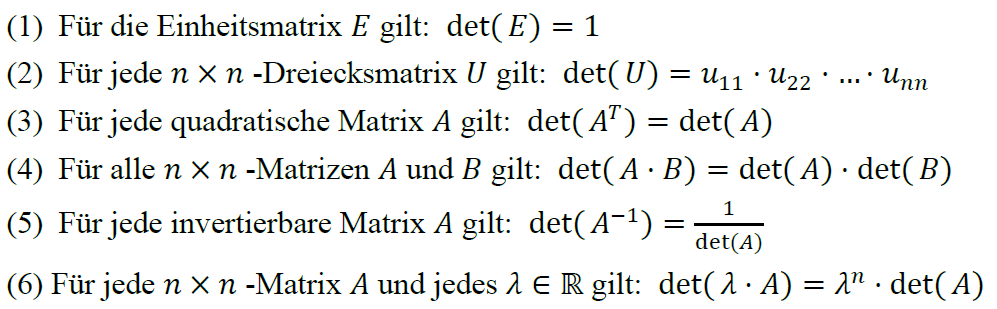
\includegraphics[scale=0.3]{det.png}}

    $2\times 2 \rightarrow det(5 \cdot A) = 5^2 \cdot det(A)$

    $3\times 3 \rightarrow det(5 \cdot A) = 5^3 \cdot det(A)$

    \WhiteSpace
    \subsection{Geometrische Interpretation der Determinante }
    {\textbf{2x2}}

    {Fläche von $\vec{a} $ und $ \vec{b} = $ Betrag von $ det \begin{vmatrix} a1 & b1  \\ a2 & b2 \end{vmatrix} $}
    {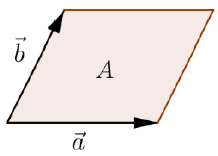
\includegraphics[scale=0.2]{2x2_det_geom.png}}




    \textbf{3x3}

    {Volumen von $\vec{a} $, $ \vec{b}$ und $\vec{c} = $ Betrag von $   det \begin{vmatrix} a1 & b1 & c1 \\ a2 & b2 & c2 \\ a3 & b3 & c3  \end{vmatrix}  $}
    {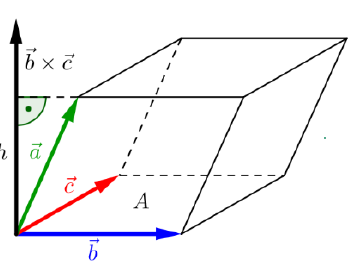
\includegraphics[scale=0.2]{3x3_det_geom.png}}
    \mbox{}


    \subsection{Matrizengleichungen}
    { \begin{center}
            \begin{tabular}{ |c|c| }
                \hline
                Grundgleichung        & Lösung                           \\ \hline
                $A \cdot X=B$         & $X = A^{-1}\cdot B$              \\
                $X \cdot A=B$         & $X = B \cdot A^{-1}\cdot $       \\
                $A \cdot X \cdot B=C$ & $X = A^{-1}\cdot C \cdot B^{-1}$ \\
                \hline
            \end{tabular}
        \end{center}}
    {\textbf{Lösung einer Matrizengleichung:} }

    {\circled{1} Wenn man eine unbekannte Matrix X ausklammert, muss X nach
        dem Ausklammern auf der Seite stehen, wo sie vorher stand:}
    $$A \cdot X + B \cdot X =(A + B) \cdot X$$

    {\circled{2}  Die Zahlen beim Ausklammern werden mit einer Einheitsmatrix
            multipliziert:}
    $$A \cdot X + 4 X =( A + 4 E) \cdot X$$
    {\circled{3} Man kann nicht durch eine Matrix dividieren, man kann aber mit
            einer inversen Matrix multiplizieren:}

        { $A\cdot X = B \to X = A^{-1} \cdot B$}

        { $X\cdot A = B \to X = B \cdot A^{-1}$}

        { $A\cdot X + 4 \cdot X = C \to (A+4E) \cdot X = C \to X = (A+4E)^{-1} \cdot C$}






    \vfill\null
    \columnbreak
    \section{Vektorräume}

    \subsection{Unterräume}
    {Eine Teilmenge U eines Vektorraums V heisst Unterraum von V wenn U selber auch ein Vektorraum ist.}

    {\textbf{Unterraumkriterien}}

    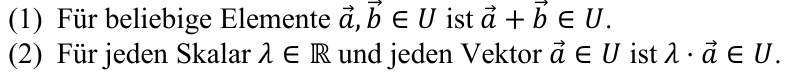
\includegraphics[scale=0.75]{unterkrit.png}
    {\textbf{Unterraumkriterien überprüfen} }

    {$ \begin{pmatrix}
                a & 0 \\
                0 & b
            \end{pmatrix} $
        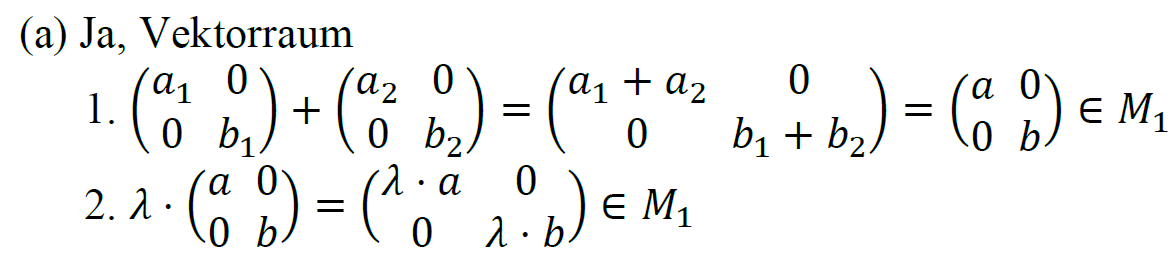
\includegraphics[scale=0.25]{unterprf1.png}}

    {$ \begin{pmatrix}
                a & 1 \\
                1 & b
            \end{pmatrix} $
        {Nein $\rightarrow$}
        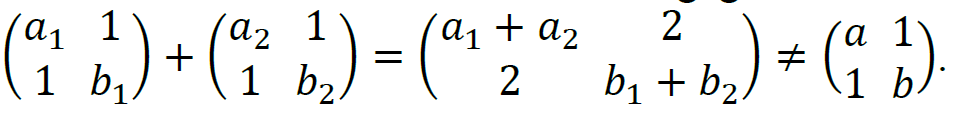
\includegraphics[scale=0.25]{unterprf2.png}}







    \subsection{Linearkombination}
    {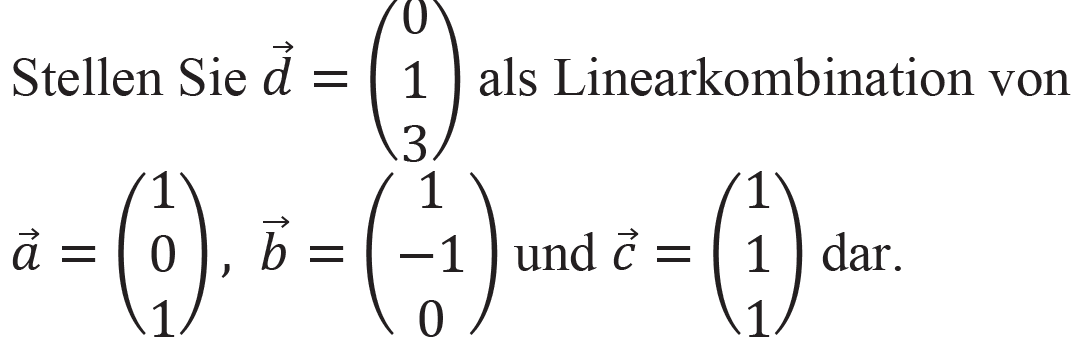
\includegraphics[scale=0.15]{linearkomba.png}}
    {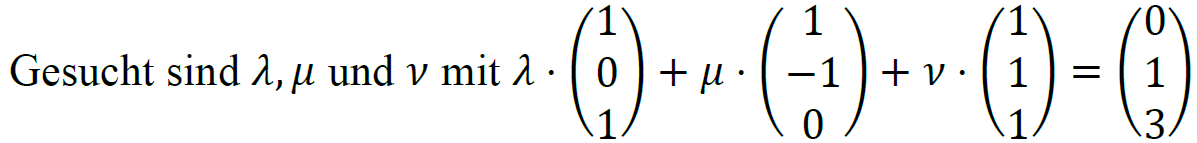
\includegraphics[scale=0.25]{linearkomb.png}}
    \subsection{Lineareabhängigkeit prüfen}
    {\textbf{Quadratische Matrix:} }

    {$det(a) = 0 \Rightarrow$ Lineare Abhängigkeit}

    {$det(a) \neq 0 \Rightarrow$  Lineare Unabhängigkeit}

    {\textbf{Nicht Quadratische Matrix:} }

    { Vektoren nebeneinander in eine Matrix schreiben $\rightarrow$ Gauss  }

    { {\small Nullzeile oder -Spalte in der Matrix} $\Longrightarrow$ Lineare Abhängigkeit der Vektoren}

    { {\small Keine Nullzeile oder-Spalte in der Matrix} $\Longrightarrow$ Lineare Unabhängigkeit der Vektoren.}
    \subsection{Linearer Spann (Lineare Hülle)}
    {Diese Menge besteht aus allen Vielfachen der Vektoren und deren Summen, ist also die Menge aller möglichen Linearkombinationen, die mit den gegebenen Vektoren gebildet werden können.}

    {$span(\vec{a},\vec{b}) = $ Ebene}

    {$span(\vec{a},\vec{b},\vec{c}) = $ eine Gerade mit Aufpunkt.}


    \subsection{Dimension}
    { Wir betrachten einen reellen Vektorraum $V$.
        Die Anzahl Vektoren, die eine Basis von $V$ bilden, heisst $Dimension$ von $V$.
    }
    {Bezeichnung: $dim(V)$}

    {\textbf{Es gilt:} }
    \begin{multicols}{2}
        {Vektorraum $\{ \vec{0} \} \rightarrow $ dim $0$}

        {$dim(span(\vec{a},\vec{b})) = 2$}

        {$dim(R^{2 \times 2})=2$}
        \columnbreak

        {dim = $rg(A)$}

        {$dim(R^{3 \times 3})=2$}

    \end{multicols}
    {\textbf{Beispiel:} }
    $$A: A^T = -A$$

    $ \begin{pmatrix}
            a & c \\
            b & d
        \end{pmatrix} =
        \begin{pmatrix}
            -a & -b \\
            -c & -d
        \end{pmatrix}$

    $\implies a=-a;$ $d=-d;$ $c=-b;$ $b=-c$

    $        \begin{pmatrix}
            0  & b \\
            -b & 0
        \end{pmatrix} \to dim() = 1$



    \subsection{Erzeugendensystem}
    {Eine Menge von Vektoren heißt Erzeugendensystem, wenn man mit ihnen alle Vektoren eines Vektorraumes durch Linearkombination erzeugen kann.}

    {\textbf{Menge von Vektoren auf Erzeugendeneigenschaft überprüfen}}

    {$\rightarrow$ Bestimmung des Rangs $rg(A)$}

    {Wenn $rg(A)$ $<$ Anzahl Zeilen($m$) $\rightarrow$ kein Erzeugendensystem}


    \subsection{Basis eines Vektorraums}
    {Eine Basis eines Vektorraumes ist ein "minimales Erzeugendensystem" des Vektorraumes. Die Vektoren einer Basis nennt man Basisvektoren.}
    {\textbf{Überprüfung, ob eine Menge von Vektoren eine Basis ist}}
    {Quadratische Matrix :$\rightarrow$ $det(A) \neq 0$}

    {Generell:}

    {\circled{1} Die Anzahl der Vektoren stimmt überein mit der Dimension des Vektorraumes.}

    {\circled{2} Die Vektoren sind linear unabhängig.}

    {\textbf{Wichtige Basen}}

    {Für $R^n$: Basis $S$ heisst $Standardbasis$ }

    {Für $P_n[x]$: Basus $M$ heisst Monombasis}
    \WhiteSpace
    \subsection{Umrechnung von Basis $B$ zur Standardbasis $S$}
    {$\vec{a} = a_1 \cdot \vec{b_1} + a_2 \cdot \vec{b_2} + a_3 \cdot \vec{b_3} ... + a_n \cdot \vec{b_n}$}

    {Beispiel:}
    {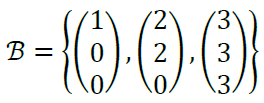
\includegraphics[scale=0.3]{umrechnung_b_to_s_bsp.png}}

    {$(7,-3,-1)$ von $B$ nach $S$}

    {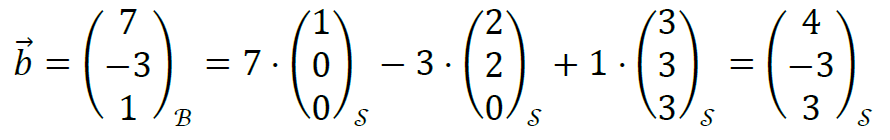
\includegraphics[scale=0.3]{umrechnung_b_to_s_lsg.png}}
    \subsection{Umrechnung von Standardbasis $S$ zur Basis $B$}
    {LGS bilden:}
    {Beispiel:}
    {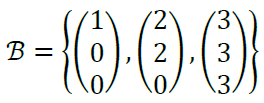
\includegraphics[scale=0.3]{umrechnung_b_to_s_bsp.png}}

    {$(2,-1,3)$ von $S$ nach $B$}

    {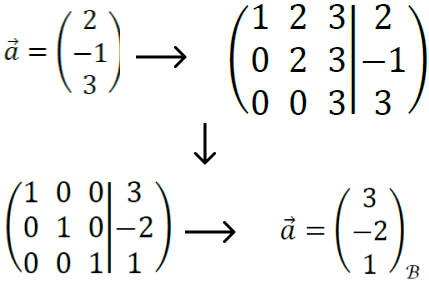
\includegraphics[scale=0.3]{Group 4.png}}
    \vfill\null
    \columnbreak
    \section{Lineare Abbildungen}
    \subsection{Definition: Lineare Abbildung}
    { Gegeben sind zwei reelle Vektorräume $V$ und $W$ (können auch identisch sein).}
    {Eine Abbildung $f:V \rightarrow W$ heisst $lineare$ $Abbildung$, wenn für alle Vektoren $\vec{x},\vec{y} \in  V$ und jeden Skalar $\lambda \in \mathbb{R} $ gilt:}

    {$(1)$ $f(\vec{x}+\vec{y})=f(\vec{x}) + f(\vec{y})$}

    {$(2)$ $f(\lambda \cdot \vec{x})=\lambda \cdot f(\vec{y})$}
    \WhiteSpace

    {Der Vektor $\vec{x} \in W$, der herauskommt, wenn $f$ auf einen Vektor $\vec{x}$ angewendet, heisst \textbf{Bild} von $\vec{x}$.}
    \WhiteSpace
    {\textbf{Beispiele:}}

    {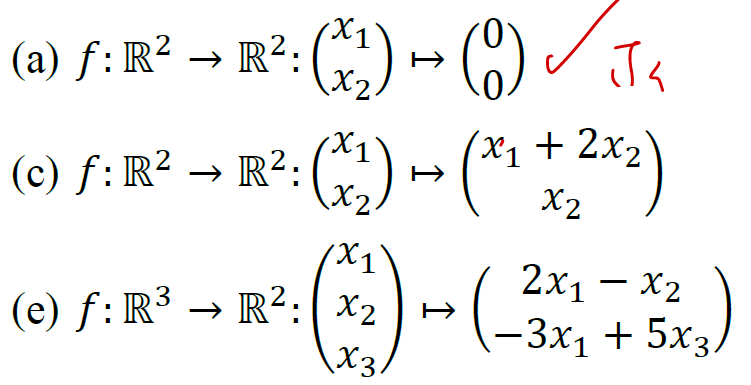
\includegraphics[scale=0.3]{lineareabbild_aufgaben.png}}

    {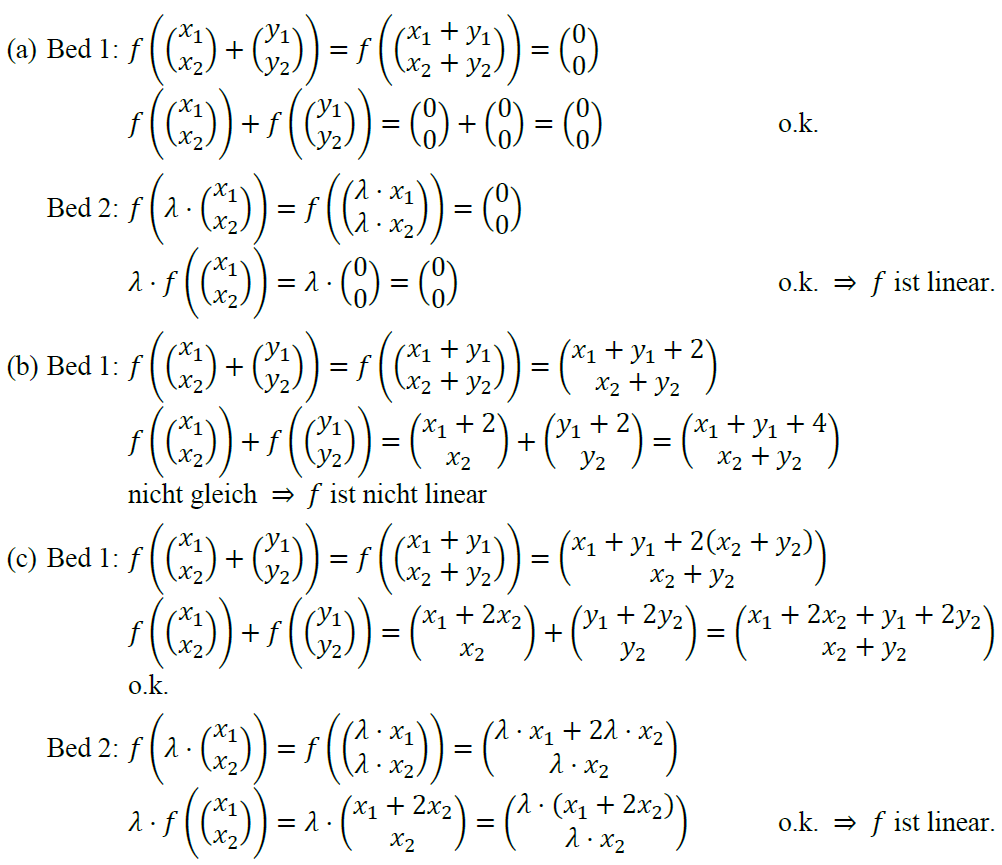
\includegraphics[scale=0.3]{lineareabbild_loesung.png}}
    \vfill\null
    \columnbreak
    \subsection{Abbildungsmatrix}
    {Bzgl. $Standardbasis$: Ablesen $\to$}

    {1.}

    {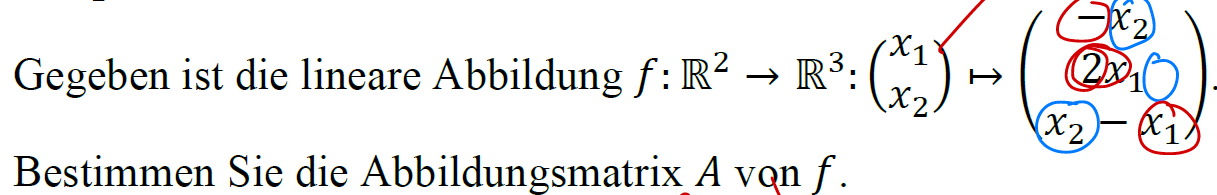
\includegraphics[scale=0.25]{abbild.png}}

    {2.}

    {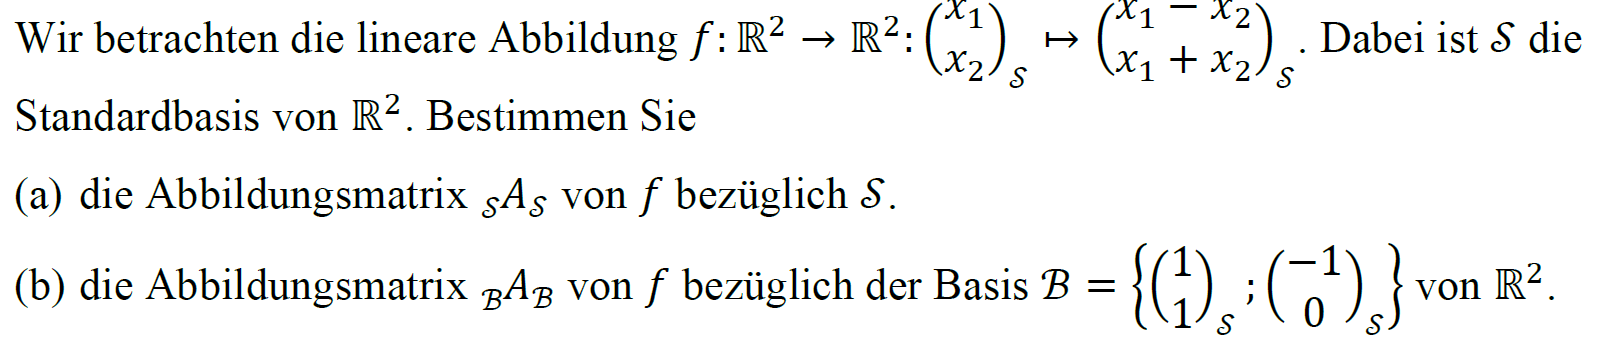
\includegraphics[scale=0.2]{abbild_1.png}}

    {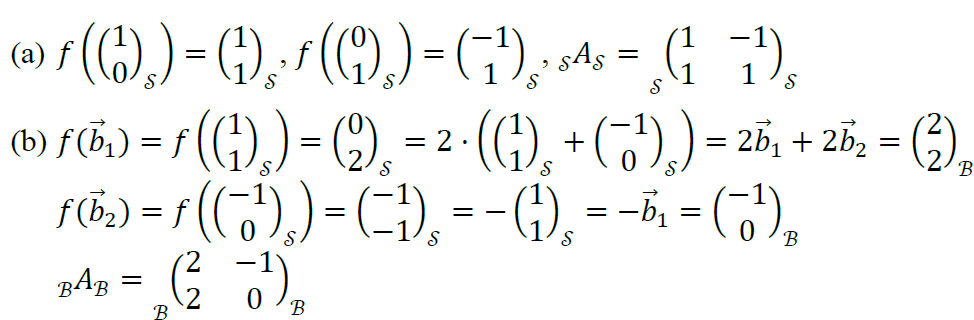
\includegraphics[scale=0.3]{abbild_3.png}}

    {\textbf{$cA_B$ Beispiel 5} }

    {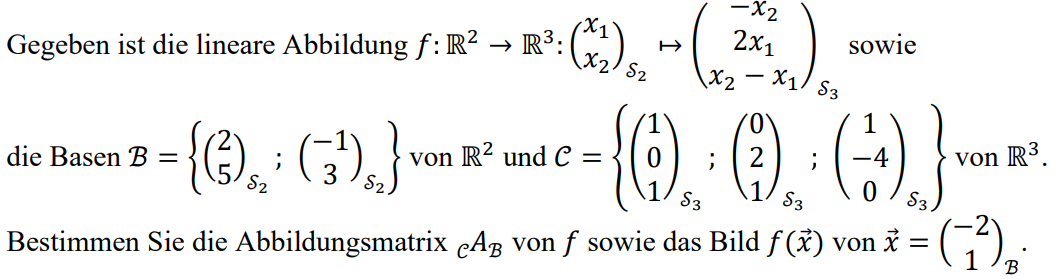
\includegraphics[scale=0.3]{bsp5.png}}

    {\circled{1} Vektoren aus $\mathcal{B} $ in $f$ einsetzen}

    {1. $ f(b_1) = f(\begin{matrix}
                2 \\
                5
            \end{matrix}) = \begin{pmatrix}
                -5 \\
                4  \\
                3
            \end{pmatrix}_S$; }{ 2. $ f(b_2) = f(\begin{matrix}
                -1 \\
                3
            \end{matrix}) = \begin{pmatrix}
                -3 \\
                -2 \\
                4
            \end{pmatrix}_S$}

    {\circled{2} dargestellt über $C$ (LGS mit $C$ und \circled{1})}


    {$( \begin{array}{rrr|cc}
                1 & 0 & 1  & -5 & -3 \\
                0 & 2 & -4 & 4  & -2 \\
                1 & 1 & 0  & 3  & 4
            \end{array})
            \to
            (\begin{array}{rrr|cc}
                    1 & 0 & 0 & {\color{red}-11} & {\color{red}-11} \\
                    0 & 1 & 0 & {\color{red}14}  & {\color{red}15}  \\
                    0 & 0 & 1 & {\color{red}6}   & {\color{red}8}
                \end{array})
        $}

    {$cA_B = \begin{pmatrix}
                {\color{red}-11} & {\color{red}-11} \\
                {\color{red}14}  & {\color{red}15}  \\
                {\color{red}6}   & {\color{red}8}
            \end{pmatrix}$}


    {\circled{3} Bild von $f(\vec{x})$ von $\vec{x} ... $}

    {$ f(b_1) = f(\begin{matrix}
                -2 \\
                1
            \end{matrix})_B = cA_B \cdot f(b_1) = f(\begin{matrix}
                -2 \\
                1
            \end{matrix})_B$}

    {$\begin{pmatrix}
                {\color{red}-11} & {\color{red}-11} \\
                {\color{red}14}  & {\color{red}15}  \\
                {\color{red}6}   & {\color{red}8}
            \end{pmatrix} \cdot \begin{pmatrix}
                -2 \\
                1
            \end{pmatrix} = \begin{pmatrix}
                11  \\
                -13 \\
                -4
            \end{pmatrix}$}

    \vfill\null
    \columnbreak
    \subsection{  Verknüpfung von linearen Abbildungen(Komposition)
    }
    {$f \to $ Abbildungsmatrix A ; $g \to $ Abbildungsmatrix B}

    {$g \circ f \to B \cdot A$  }

    {$f \circ g \to A \cdot B$  }

    {Die Matrix der Abbildung, die zuerst ausgeführt wird, steht $rechts$}

    \subsection{ lineare Abbildungen in der Ebene}
    {$\rightarrow $ $!$ normieren nicht vergessen $!$ $\leftarrow$}
    {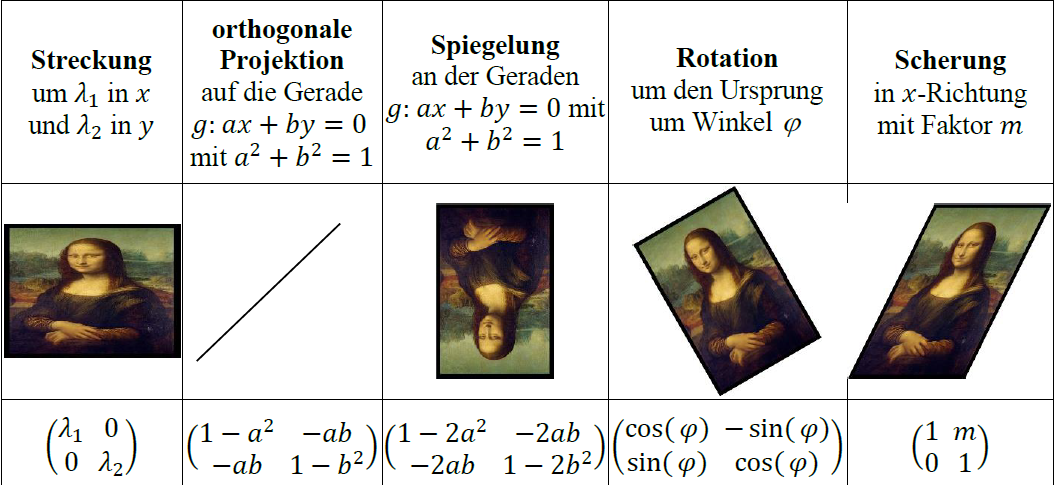
\includegraphics[scale=0.325]{wichtige lineare Abbildungen in der Ebene.png}}

    \subsection{ linearen Abbildungen im Raum}
    {$\rightarrow $ $!$ normieren nicht vergessen $!$ $\leftarrow$}
    {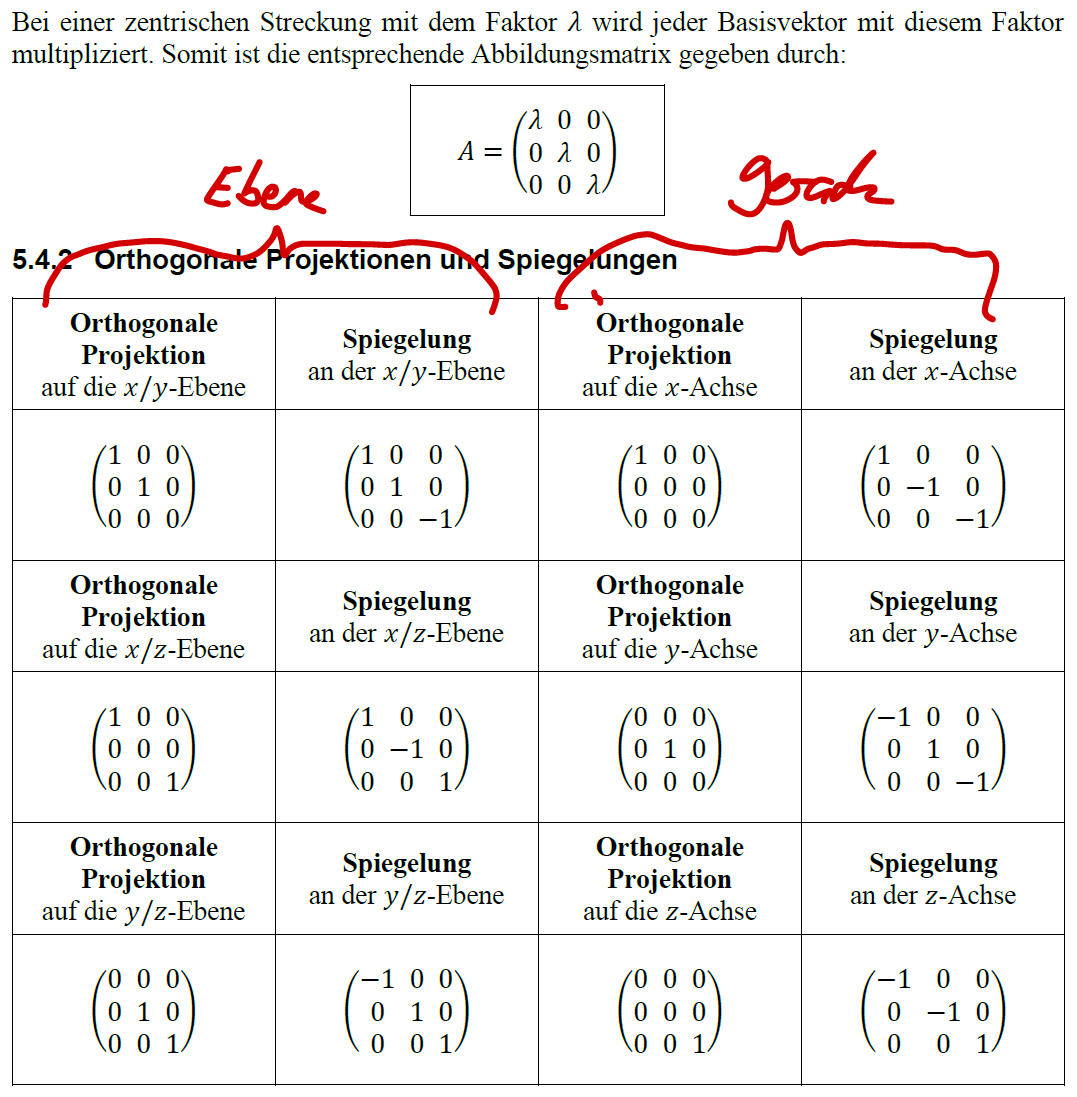
\includegraphics[scale=0.325]{linearen Abbildungen im Raum.png}}

    \vfill\null
    \columnbreak
    \subsection{ Rotationen}

    {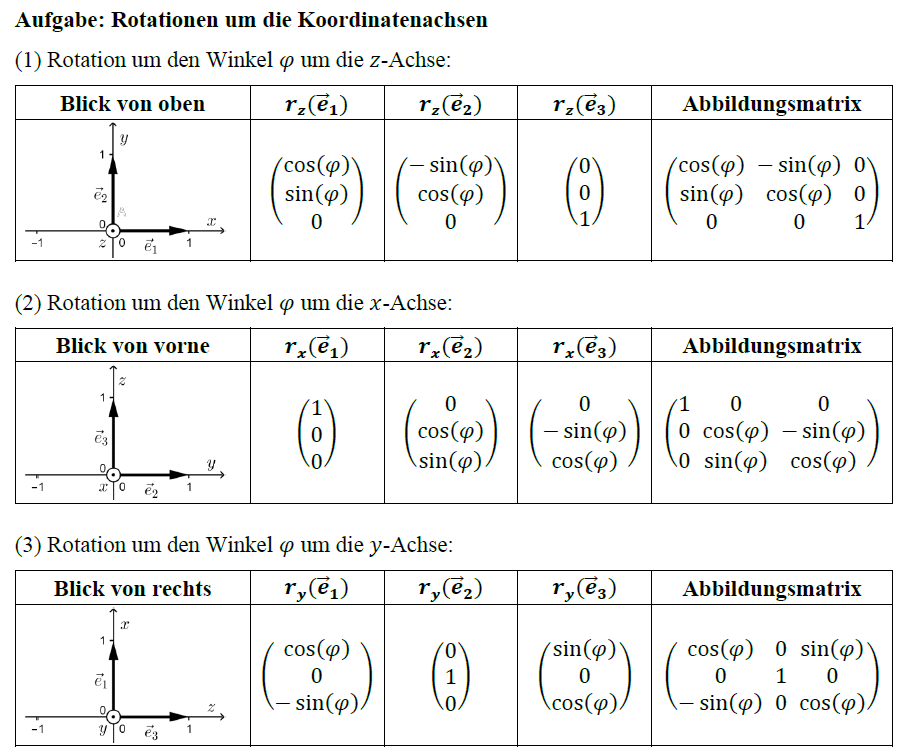
\includegraphics[scale=0.3825]{rotation.png}}

    {Rotation um eine allgemeine Achse durch den Ursprung}
    {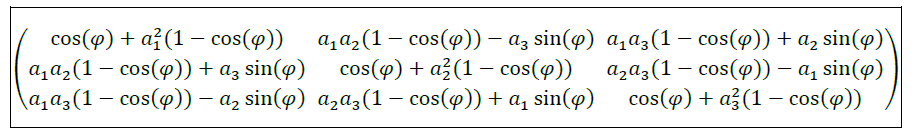
\includegraphics[scale=0.325]{rotation_2.png}}

    \subsection{ Kern einer Matrix}
    {\textbf{Definition:} Der Kern $ker(A)$ einer $m\times n$ -Matrix $A$ ist die Lösungsmenge des homogenen linearen
        Gleichungssystems: $$A\cdot \vec{x} = \vec{0}$$}
    {$$\det(A) \neq 0 \quad \rightarrow \quad \text{Kern(A)}=\{0\} \quad \text{trivial}$$}
    {$$\det(A)=0 \quad \rightarrow \quad \text{Kern(A) ist nicht trivial}.$$}

    {$\rightarrow$ Abbildungsmatrix  $\rightarrow$ Lösen durch LGS}

    {Beispiel 1:}

    {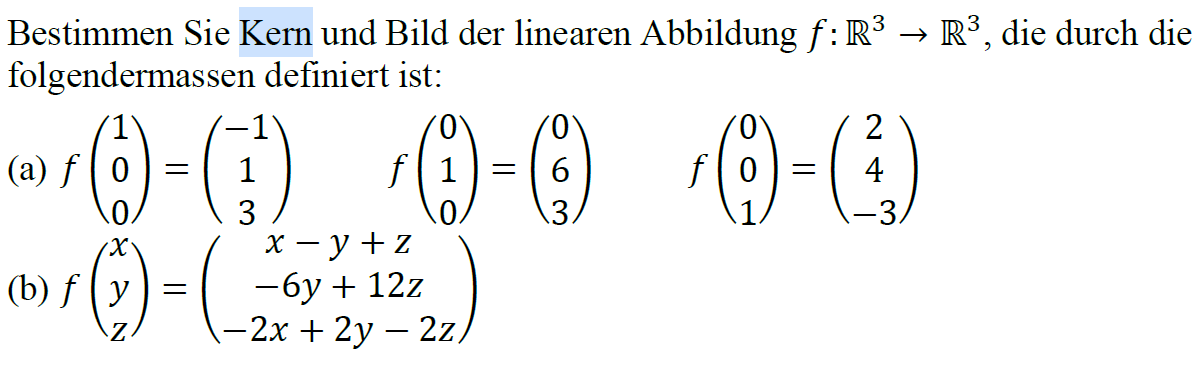
\includegraphics[scale=0.28]{Kern.png}}

    {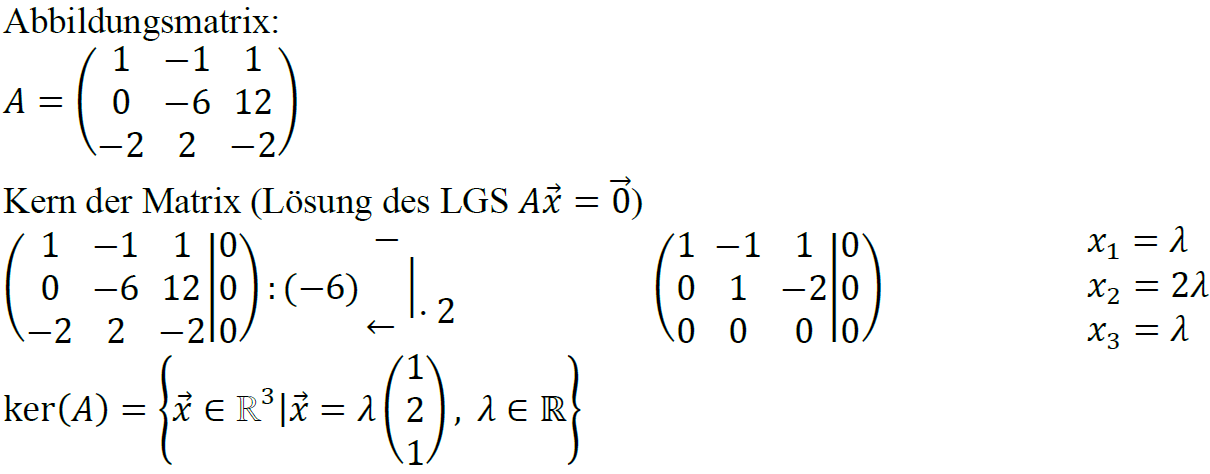
\includegraphics[scale=0.28]{Kern_2.png}}


    
    {Beispiel 2:}

    {\includegraphics[scale=0.28]{Kern_3.png}}

    {\includegraphics[scale=0.28]{Kern_4.png}}

    \subsection{ Bild einer Matrix}
    {Wir multiplizieren eine Matrix $A$  mit einem Vektor $\vec{x}$
        und erhalten den Lösungsvektor $\vec{b}$.}

    {Das Bild einer Matrix gibt an, welche Menge an Vektoren als Lösungen auftreten können.}

    {$\to$ Die linear unabhängigen Spalten einer Matrix heißen Bild der Matrix.}



    {\circled{1} Matrix in obere Dreiecksmatrix umwandeln}

    {\circled{2} Linear unabhängige Spalten mithilfe der Köpfe bestimmen}

    {\circled{3} Lösung aufschreiben}

    {$A =  \begin{pmatrix} 1 & 3 & 2 \\ 2 & 4 & 4 \\ 3 & 5 & 6 \end{pmatrix}$   {\circled{1}$\to$ $\begin{pmatrix} 1 & 3 & 2 \\ 0 & -2 & 0 \\ 0 & 0 & 0 \end{pmatrix}$}}

    {\circled{2} $\begin{pmatrix} {\color{blue}1} & 3 & 2 \\ 0 & {\color{blue}-2} & 0 \\ 0 & 0 & 0 \end{pmatrix} \rightarrow$   $\begin{pmatrix} {\color{red}1} & {\color{red}3} & 2 \\ {\color{red}2} & {\color{red}4} & 4 \\ {\color{red}3} & {\color{red}5} & 6 \end{pmatrix}$}

    {Da sich die Köpfe in der 1. und 2. Spalte befinden, sind diese beiden Spalten der ursprünglichen (!) Matrix die linear unabhängigen Spalten.}



    {\circled{3} $\text{img}(A) = \left\langle \begin{pmatrix} 1 \\ 2 \\ 3 \end{pmatrix}, \begin{pmatrix} 3 \\ 4 \\ 5 \end{pmatrix} \right\rangle$}

    Beispiel aus der Aufgabe von "Kern der Matrix"

    {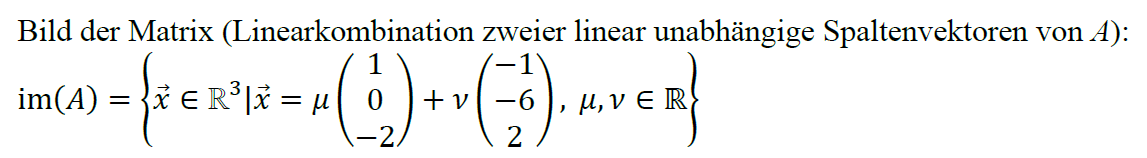
\includegraphics[scale=0.28]{bild.png}}

    \subsection{Basiswechsel von $S$ nach $B$}

    ${}_{B}T_{S} = ({}_{S}T_{B})^{-1}$

    ${}_{S}A_{S} = {}_{S}T_{B} \cdot {}_{B}A_{B} \cdot {}_{B}T_{S}$

    ${}_{B}A_{B} = {}_{B}T_{S}  \cdot {}_{S}A_{S} \cdot {}_{S}T_{B}$



\end{multicols*}




\end{document}
